% 11/11/2020 - First round of corrections: added Manolo's corrections
% 15/11/2020 - Second round of corrections: added Thomas (new) & Ray corrections
% 15/11/2020 - Grammarly
% 16/11/2020 - Corrected images

\begin{refsection}
\chapter{Effect of optical imperfections on an X-ray beam}
\label{sec:effect_optical_imperfections}

The effects of the optical imperfections modelled and measured in Chapter~\ref{sec:measuring} to an X-ray beam are presented in this chapter in terms of fully- and partially- coherent simulations were done with the \textit{SRW} code and the specially developed Python library for refractive optics (barc4RefractiveOptics) presented in Chapter~\ref{sec:modelling}. The fully-coherent simulations include the beam-caustics and the point-spread function (PSF - intensity and phase) for the system being modelled. Partially-coherent simulations comprise the beam characteristics at the image plane and the beam profile at selected positions along the optical axis. These simulations are used to extensively evaluate the performance of commercially available Be lenses; compare the validity of individually measured and artificially stacked lenses against the stack measurement; and the different effects of distinct spatial frequency ranges in figure errors to the optical performance of the CRL.

%-------------------------------------------------------------------------
%-------------------------------------------------------------------------
\section{Lenses and lens stacks}\label{sec:lens_descripiton}
%-------------------------------------------------------------------------
%-------------------------------------------------------------------------
The modelled lenses are 2D-Be lenses with a nominal radius of $R=50~\mu\text{m}$ chosen as representative of lenses used widely at beamlines at many synchrotrons - see Fig.~\ref{fig:1D2D_lenses}(b) and (d). Such lenses have typically 1~mm thickness and are held in a 2~mm thick lens frame (newer ones 1.6~mm thick), which delimits the spacing $\Delta\text{s}=2~$mm between individual lenses in Eq.~\ref{eq:TE_CRL_MS_ERR}. Those lenses can be manufactured with wall thickness in the range of $\sim30~\text{to}~40~\mu\text{m}$. Applying Eq.~\ref{eq:A}, one obtains $A_{\diameter}\le440 \mu\text{m}$. At 8~keV, the energy used for the simulations, the index of refraction for beryllium is $n=1-5.318\times10^{-6}+i\cdot2.071\times10^{-9}$ and the corresponding intensity transmission of this lenslet is shown in Fig.~\ref{fig:EffectiveAperure}(a). Applying Eq.~\ref{eq:CRL_classic} with $N=1$, one obtains the focal length for a single lens: $f_{\text{lens}}=4.701$~m. The lens stacks used are composed of $N=10$ lenses, except for the stacks used in the simulations shown in Fig.~\ref{fig:CDn01-05-10}, where the number of lenses $N$ varies ($N=1,5,10$).  The lens stack focal distance can be obtained by applying Eq.~\ref{eq:CRL} with $N=10$ and $L=(N-1)\cdot2~\text{mm}=18~\text{mm}$: $f_{\text{CRL}}=473~{\text{mm}}$, giving a magnification of approximately $126:1$ ($M\approx8\times10^{-3}$ for a source 60~m away from the centre of the CRL) and a diffraction-limited spot size (Eq.~\ref{eq:PSF}) of $\sim200~\text{nm}$. The error profiles used for the simulations have been described in \S\ref{sec:single_lens}~-~\textit{\nameref{sec:single_lens}} when measured individually and in \S\ref{sec:lens_stack}~-~\textit{\nameref{sec:lens_stack}} when measured as a 10-element stack.

The comparison between the simulations using 10 different individually measured lenses against simulations using metrology from a lens stack composed of those very same lenses is shown in Fig.~\ref{fig:CDn_vs_CDnStack} for lenses L01-L10 and in Fig.~\ref{fig:CDo_vs_CDoStack} for the lenses L11-L20. Simulations of a single lens (L01), five stacked lenses (L01-L05) and ten stacked lenses (L01-L10) are used to investigate the deterioration of the X-ray beam profile upon stacking lenses. These can be seen in Fig.~\ref{fig:CDn01-05-10}. The effect of different spatial frequency ranges in the X-ray beam is shown in Fig.~\ref{fig:CDnFF_LF_HH}, where the performance of the accumulated figure error profile of lenses L01-L10 is compared against the performance of its decomposition in Zernike circular polynomials and the residues of such fit. Finally, the lens stack formed by individually measured lenses L01-L10 is meticulously studied under fully- and partially-coherent illumination. Figure~\ref{fig:CDnS} shows transverse cuts along the optical axis, the beam caustics, PSF (intensity and phase) and the demagnified image of the X-ray source (CPMU18\footnote{Cryogenic Permanent Magnet Undulator.}).

%-------------------------------------------------------------------------
%-------------------------------------------------------------------------
\section{Software and computing infrastructure}\label{sec:SRW}
%-------------------------------------------------------------------------
%-------------------------------------------------------------------------

All simulations presented here were done using the "Synchrotron Radiation Workshop" (SRW) [\cite{Chubar1998}]\footnote{Available at \url{https://github.com/ochubar/srw}}, as it conveniently offers the possibility of fully- and partially-coherent calculations\footnote{See \S\ref{sec:wave_propag}~-~\textit{\nameref{sec:wave_propag}} and \S\ref{sec:partially_coherent}~-~\textit{\nameref{sec:partially_coherent}}.}, and presents parallelisation with the MPI standard [\cite{Chubar2011}]. Fully coherent calculations were done using a single CPU of an Intel(R) Xeon(R) CPU E5-2680 v4 @ 2.40GHz, while partial coherent simulations used 28 CPUs of the same type (NICE OAR cluster at the ESRF). The specially developed python library for dealing with the refractive lenses with the addition of optical imperfections (barc4RefractiveOptics) presented in Chapter~\ref{sec:modelling} was also used in the simulations.

\begin{figure}[t]
        \centering
        {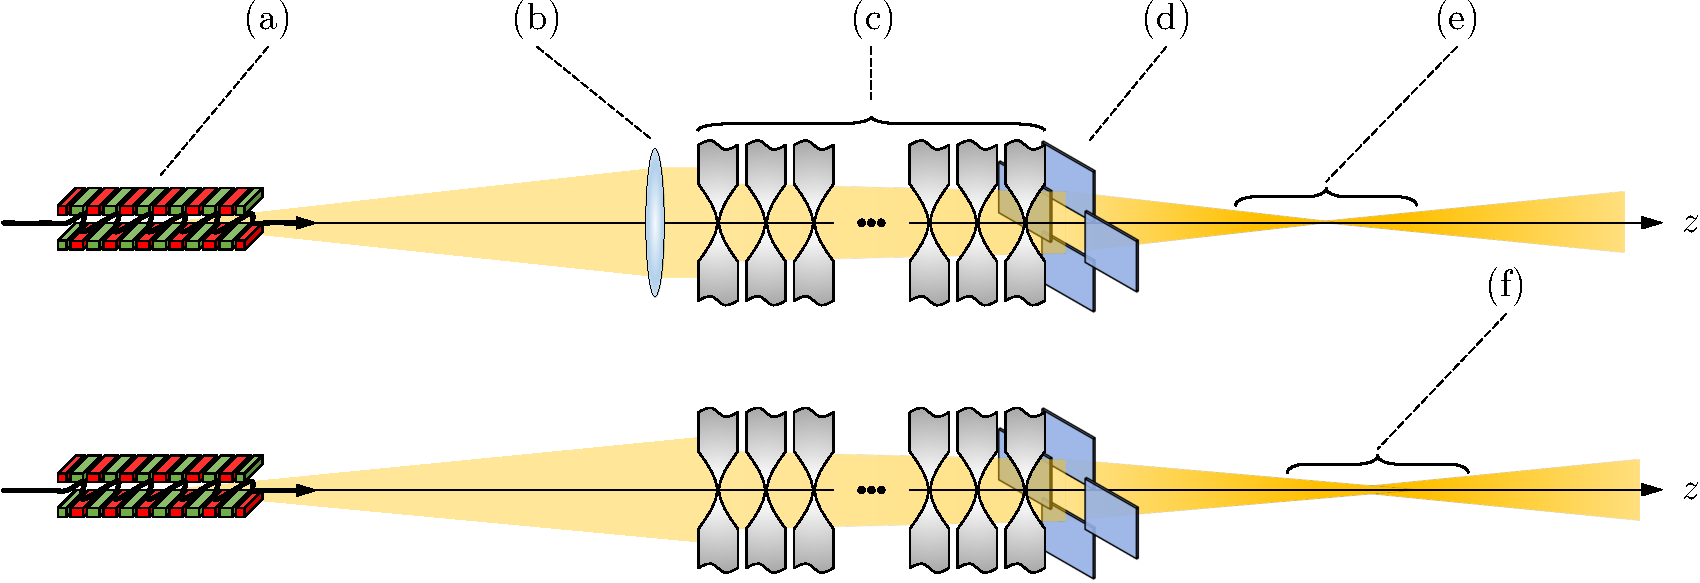
\includegraphics[width=0.8\linewidth]{figures/ch05/optical_setups.pdf}}
        \caption[Beamlines for coherent- and partially-coherent simulations]{\textbf{top row}: beamline used for  \S\ref{sec:coherent_sim}~-~\textit{\nameref{sec:coherent_sim}}. \textbf{bottom row}: beamline used for  \S\ref{sec:partcoherent_sim}~-~\textit{\nameref{sec:partcoherent_sim}}. (a) shows the X-ray source: a CPMU18 undulator. An (b) ideal parabolic phase element with radius of curvature $R=-60~$m is placed 60~m downstream the radiation source to give the illumination a near-plane phase - cf. Eq.~\ref{eq:planewave}. This ideal element is only present for the fully-coherent simulations. The lenses being studied are shown in (c). They are immediately followed by a set of (d) slits to ensure the same geometric aperture for all simulations and aid direct calculation of the Strehl ratio. For the fully-coherent simulations, the beam-caustic range is shown in (e) and the PSF is calculated at the centre of it. For the partially-coherent simulations, the beam profile evolution along the optical axis is shown in (f) and the beam characteristics at the focal position are calculated at its centre. 
        }\label{fig:optical_setups}
\end{figure}

%-------------------------------------------------------------------------
%-------------------------------------------------------------------------
\section{Fully coherent simulations}\label{sec:coherent_sim}
%-------------------------------------------------------------------------
%-------------------------------------------------------------------------

For this set of simulations, the X-ray source is a filament electron-beam passing through a CPMU18 undulator with 111 magnetic periods, $\Lambda=18$~mm magnetic period and magnetic field $B=0.9863~$T emitting a 1$^\text{st}$ harmonic photon beam at 8~keV (resonance). The photon source size and divergence are given by the specific radiation
pattern size and divergence of the insertion device and the emission is fully coherent\footnote{cf. \S\ref{sec:optical_coherence}~-~\textit{\nameref{sec:optical_coherence}}.}  - see \S\ref{sec:brilliance}~-~\textit{\nameref{sec:brilliance}}. At 60~m away from the source, the beam footprint\footnote{Although commonly approximated by Gaussian distributions, undulator emission does not possess Gaussian distribution not even at resonance. Please, refer to footnote \ref{note:und_prof} in \S\ref{sec:brilliance}~-~\textit{\nameref{sec:brilliance}} for a deeper discussion on the emission profile of undulator radiation and for further references.} is large enough to illuminate the full geometric aperture of a lens with $A_{\diameter}\le440 \mu\text{m}$ with an intensity variation of 2\% (centre to the edge). The illumination profile in conjunction with the transmission profile of the lenses being modelled (Fig.~\ref{fig:EffectiveAperure}) allows classifying such systems as apodised. In the paraxial approximation, the radiation phase for this source is dominated by a quadratic phase term [\cite{Chubar1999, Chubar2001b, Chubar2019}]. At the position along the optical axis where the intensity is calculated, this quadratic phase term can be compensated by placing an ideal lens with focal length $f=-60~$m. This ensures a plane-wave illumination (Eq.~\ref{eq:planewave}) downstream the ideal element, which is used to illuminate the different CRL models being studied. The lens stack and imperfect lenses are modelled using the CRL multi-slice approach with errors added described by Eq.~\ref{eq:TE_CRL_MS_ERR} and shown in Fig.~\ref{fig:models}(c) in \S\ref{sec:CRL_modelling}~-~\textit{\nameref{sec:CRL_modelling}}. The evaluation of the effect of optical imperfections on an X-ray beam is performed at the image plane of the focusing system and in its vicinity. The beamline used for the fully-coherent simulations is shown in  Fig.~\ref{fig:optical_setups}.

\begin{table}[h]
\caption[FWHM of the PSF for the simulated models in Figs.~\ref{fig:CDn_vs_CDnStack}-\ref{fig:CDnS}]{Summary of the beam sizes in FWHM for various CRL models. The extended source image sizes are taken from the partially coherent simulations averaging the intensity of 10$^{4}$ wavefronts.}\label{tab:beamsizes}\small

\centering
\begin{tabular}{lrcccc}\hline \hline
&                        &\multicolumn{2}{c}{\textbf{PSF} (nm)}   &\multicolumn{2}{c}{\textbf{source image} (nm)}\\
&\textbf{lens model}     &hor.           &ver.                    &hor.            &ver. \\ \cline{2-6}
&analytic equations       &\multicolumn{2}{c}{223.3}           &603.8           &241.7 \\
&ideal CRL               &217.5          &218.7                   &626.4           &247.5 \\ \hline
Fig.~\ref{fig:CDn_vs_CDnStack} &L01-L10  &208.8  &210.1           &680.1           &254.4 \\
&stack 01                &206.2          &219.5                   &692.0           &254.1\\ \hline
Fig.~\ref{fig:CDo_vs_CDoStack} &L11-L20  &194.7  &197.5           &835.1           &374.8 \\
&stack 02                &192.1          &203.1                   &748.6           &268.9 \\ \hline
Fig.~\ref{fig:CDn01-05-10}&single ideal lens  &\multicolumn{2}{c}{1959.4}   & -    & -\\
&L01                     &1954.0         &1957.3                  & -              & - \\
&five ideal stacked lenses  &\multicolumn{2}{c}{401.3}            & -              & - \\
&L01-L05                 &384.5       &399.0                      & -              & - \\ \hline
Fig.~\ref{fig:CDnFF_LF_HH} &LF L01-L10  &214.8     &206.0         & 731.4          &263.7 \\
&HF L01-L10              &225.1      &231.6                       & 637.5          &246.1 \\
\hline \hline
\end{tabular}
\end{table}{}

%-------------------------------------------------------------------------
%-------------------------------------------------------------------------
\subsection{The PSF: ideal focusing}\label{sec:psf_sim}
%-------------------------------------------------------------------------
%-------------------------------------------------------------------------

After passage through the CRL model being studied, the plane wave used for illuminating the optical system will develop a quadratic phase term that has a curvature radius equivalent to the effective focal distance of the optical system, which is given by Eq.~\ref{eq:CRL}. The propagation of the wavefront from the exit pupil of the CRL to the image plane located at a focal length distance is equivalent to an optical 2D-Fourier transform of the system pupil function. The PSF of the optical system corresponds to the squared modulus of this Fourier transform, which is the wavefront intensity at the focal plane, considering a plane wave illumination [\cite[\textit{\S2.3.1} \& \textit{\S6.2}]{Goodman2017}]. The phase of the propagated field at the focal position, the normalised PSF and relative intensities of the aberrated PSF normalised to the ideal case (Strehl ratio) are shown in Figs.~\ref{fig:CDn_vs_CDnStack}-\ref{fig:CDo_vs_CDoStack}(b-c) and (e);  Fig.~\ref{fig:CDn01-05-10}(b)-(d); Fig.~\ref{fig:CDnFF_LF_HH}(b-c) and (e); and Fig.~\ref{fig:CDnS}(d)-(e). The calculated FWHM of the central lobe of the PSF for the simulated models presented in Figs.~\ref{fig:CDn_vs_CDnStack}-\ref{fig:CDnS} are displayed on Table~\ref{tab:beamsizes} and the respective Strehl ratio, compiled in Table~\ref{tab:Strehl}.

\begin{table}[t]
\caption[Strehl ratio for the simulated models in Figs.~\ref{fig:CDn_vs_CDnStack}-\ref{fig:CDnS}]{Comparison of the Strehl ratio for the simulated models in Figs.~\ref{fig:CDn_vs_CDnStack}-\ref{fig:CDnS}}\label{tab:Strehl}%\small
\resizebox{\columnwidth}{!}{
\centering
\begin{tabular}{lrcccccc}\hline \hline
&\textbf{lens model}     &$\sigma_z$ ($\mu$m)     &$S_{\text{a}}$ (Eq.~\ref{eq:Strehl})  &$S_{\text{b}}$  (Eq.~\ref{eq:Marechal}) &$S_{\text{c}}$  (Eq.~\ref{eq:Mahajan}) &$S_{\text{ratio coh.}}$ &$S_{\text{ratio part.-coh.}}$ \\ \cline{2-8}
Fig.~\ref{fig:CDn_vs_CDnStack} &L01-L10  &4.84  &0.067      &0.285 &0.393  &0.394          &0.409 \\
&stack 01                                &5.75  &-          &0.054 &0.215  &0.374          &0.375\\ \hline
Fig.~\ref{fig:CDo_vs_CDoStack} &L11-L20  &6.28  &-          &0.007 &0.160  &0.185          &0.211 \\
&stack 02                                &6.48  &-          &0.001 &0.142  &0.243          &0.247 \\ \hline
Fig.~\ref{fig:CDn01-05-10} &L01          &0.57  &0.985      &0.985 &0.985  &0.981          & -  \\
&L01-L05                                 &2.67  &0.669      &0.696 &0.718  &0.684          & - \\ \hline
Fig.~\ref{fig:CDnFF_LF_HH} &LF L01-L10   &4.36  &0.116      &0.311 &0.413  &0.335          &0.359 \\
&HF L01-L10                              &2.18  &0.779      &0.791 &0.802  &0.796          &0.778 \\
\hline \hline
\end{tabular}
}
\end{table}{}

%-------------------------------------------------------------------------
%-------------------------------------------------------------------------
\subsection{The beam caustics}\label{sec:caustics_sim}
%-------------------------------------------------------------------------
%-------------------------------------------------------------------------

The beam characteristics at the image plane are very important and the PSF simulations in Figs.~\ref{fig:CDn_vs_CDnStack}~to~\ref{fig:CDnS} show obvious differences between ideal and aberrated focusing of CRLs. It is necessary, however, to complement this with investigations of the effect of optical imperfections away from the focal position, especially because several experimental applications may use a defocused beam for obtaining a larger footprint. To get an overview of the beam evolution up- and downstream of the focal position, one can propagate the wavefront along the optical axis and for each position extract a cross-section of the beam. This will be referred to as the beam caustic\footnote{Strictly speaking, the beam caustic is the envelope of light rays after passing through an optical element - see p.~60 [\cite{Lawrence1972}]. A more comprehensive theory of caustics in optics is given by [\cite{Kravstov1999, Nye1999}].}. The beam caustics are shown in Figs.~\ref{fig:CDn_vs_CDnStack}-\ref{fig:CDnFF_LF_HH}(a); and Fig.~\ref{fig:CDnS}(c). The beam cross-section for selected positions along the beam optical axis can be seen in Fig.~\ref{fig:CDnS}(b). The vertical cuts were taken at $x=0$. The zero position along the optical axis is given by the distance from the centre of the CRL to the image plane, position where the PSF is calculated. To calculate the beam caustics, the wavefront was propagated from 10~mm upstream of the focal position to 10~mm downstream in 4001 equally spaced steps along the optical axis.

%-------------------------------------------------------------------------
%-------------------------------------------------------------------------
\section{Partially coherent simulations}\label{sec:partcoherent_sim}
%-------------------------------------------------------------------------
%-------------------------------------------------------------------------

The PSF and beam caustic simulations presented previously are both fully-coherent calculations. They present the focusing of a perfect plane wavefront to a diffraction-limited spot. This shows the intrinsic limitations of the optical system, but inherently neglects the effects of an extended and partially coherent source.

%-------------------------------------------------------------------------
%-------------------------------------------------------------------------
\subsection{X-ray source}\label{sec:source_sim}
%-------------------------------------------------------------------------
%-------------------------------------------------------------------------
The emission of a single electron passing through an undulator (filament beam) is fully coherent. By changing the electron initial conditions (positions, direction and energy), propagating the emission of this electron through the beamline and adding up intensities, one can simulate partially coherent radiation if the electron beam phase space (5D) is sufficiently sampled as discussed in \S\ref{sec:partially_coherent}~-~\textit{\nameref{sec:partially_coherent}} - see also [\cite{Chubar2011}]. 

For this section, a hypothetical beamline operating on the new Extremely Brilliant Source (ESRF-EBS) magnetic lattice [\cite{orangebook}] is implemented. This beamline is shown in Fig.\ref{fig:optical_setups}. The beamline sits on a straight section and has a CPMU18 undulator as an insertion device. The undulator was tuned to its first harmonic at 8~keV for all simulations. The photon source size is $\sim71.9\times12.4~\mu\text{m}^2$ and its divergence $\sim17.7\times14.7~\mu\text{rad}^2$ (FWHM, horizontal vs. vertical). The first optical element was placed 60~m downstream of the centre of the undulator to ensure a beam footprint larger than the geometric aperture of the CRL being studied ($A_{\diameter}\sim440~\mu\text{m}$) and a constant intensity over it. The transverse coherence length $\Delta_{\textbf{cl}_{\perp}}$ at the entrance of the optical system is estimated to be $\sim60\times448~\mu\text{m}^2$ (FWHM, horizontal vs. vertical), from the calculation of the complex degree of spatial coherence\footnote{see \textit{Spatial coherence} in \S\ref{sec:optical_coherence}~-~\textit{\nameref{sec:optical_coherence}}.} $j(\textbf{r}_1,\textbf{r}_2)$ - see Fig.~\ref{fig:CDoC}. This difference between the horizontal and vertical transverse coherence length is a direct consequence of the photon-source size asymmetry and the van-Cittert-Zernike theorem [\cite[\textit{§4}]{Geloni2008}]. If there is no spatial filtering, the horizontal direction is less coherent than in the vertical, leading to stronger blurring of the image in the less coherent direction [\cite[\textit{\S7.5}]{Goodman2017}]. 

\begin{figure}[t]
        \centering
        {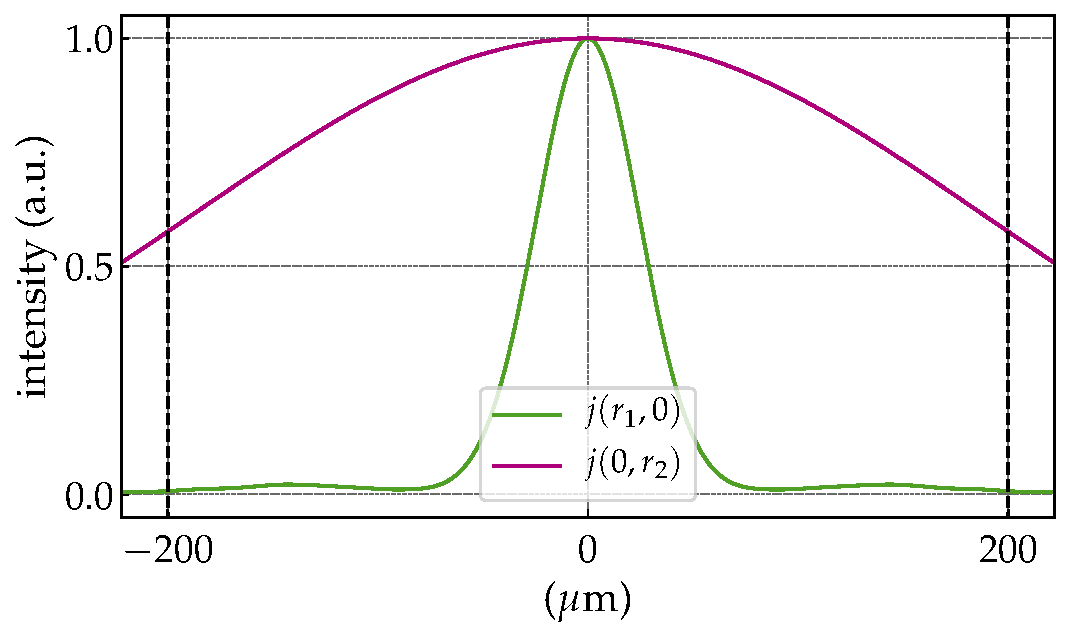
\includegraphics[height=4cm]{figures/ch05/source/CdoC.pdf}}
        \caption[Complex degree of coherence]{Horizontal ($j(\textbf{r}_1,0)$) and vertical ($j(0,\textbf{r}_2)$) cuts of the complex degree of coherence function immediately before the CRL - see \S\ref{sec:source_sim}~-~\textit{\nameref{sec:source_sim}}. The vertical dashed lines indicate the geometric aperture used for the simulations. 
        }\label{fig:CDoC}
\end{figure}
%-------------------------------------------------------------------------
%-------------------------------------------------------------------------
\subsubsection*{On the convergence of the simulations}
%-------------------------------------------------------------------------
%-------------------------------------------------------------------------
In a conservative approach, the partially coherent simulations presented here were done using 10$^{4}$ wavefronts to ensure convergence.
The convergence of the partially-coherent simulations is connected to the sampling of the electron distribution $f(s,s',\gamma_e)$, where each electron in a bunch has a different initial condition in terms of position $s=(x_e,y_e,z_e=0)$, direction $s'=(x'_e,y'_e)$ and energy $\gamma_e$ - see \textit{Physical-optics-based methods} in \S\ref{sec:partially_coherent}~-~\textit{\nameref{sec:partially_coherent}}. Commonly used criteria for evaluating the quality of the sampling of the electron distribution are \textit{i}-) smooth and homogeneous illumination at the aperture of the first optical element;  \textit{ii}-) the beamline overall transmission; and \textit{iii}-) the smoothness of the beam profile at the end of the optical system prior to taking into account optical imperfections [\cite{SanchezdelRio2019}].%\todo{Fig.~\ref{fig:ME_convergence} shows the sampling of the function $f(s,s',\gamma_e)$ for the ESRF-EBS, the old ESRF-low $\beta$ and the old ESRF-high $\beta$ straight sections.}

% \begin{table}[t]
% \caption[Electron-beam parameters for the ESRF-ESB, the old ESRF-low $\beta$ and the old ESRF-high $\beta$ straight sections]{\todo{Electron-beam parameters for the ESRF-ESB, the old ESRF-low $\beta$ and the old ESRF-high $\beta$ straight sections.}}\label{tab:E_beam_param}
% \centering
% \begin{tabular}{rccc}

% \end{tabular}
% \end{table}{}

%-------------------------------------------------------------------------
%-------------------------------------------------------------------------
\subsection{Beam characteristics at the focal position}\label{sec:source_image_sim}
%-------------------------------------------------------------------------
%-------------------------------------------------------------------------

The image of the extended X-ray source is similar to the convolution between the geometrically demagnified image of the source and the 2D-PSF of the imaging system, provided the beam is not strongly cropped anywhere in the beamline being simulated. For the cases being studied here, the beam footprint at the entrance pupil of the CRL system is several times larger than the geometric aperture of a single lens and this convolution approach is not valid, hence the necessity of the partially-coherent simulations for imaging the source in the centre of the CPMU18. Figures~\ref{fig:CDn_vs_CDnStack}-\ref{fig:CDo_vs_CDoStack}(e), Fig.~\ref{fig:CDnFF_LF_HH}(e) and Fig.~\ref{fig:CDnS}(f) show the normalised demagnified image of the undulator photon source while Table~\ref{tab:beamsizes} presents the horizontal and vertical FWHM for those simulations. Figures~\ref{fig:CDn_vs_CDnStack}-\ref{fig:CDo_vs_CDoStack}(f) and Fig.~\ref{fig:CDnFF_LF_HH}(f) show graphical representation of the intensity profiles of the different focusing conditions on a normalised scale where the ideal diffraction-limited focusing peak intensity is 1. Consequently, the peak intensities of the other profiles give the Strehl irradiance ratios for the corresponding configuration. These values are compiled in Table~\ref{tab:Strehl}.

%-------------------------------------------------------------------------
%-------------------------------------------------------------------------
\subsection{Beam profile evolution along the optical axis}\label{sec:partcaustics_sim}
%-------------------------------------------------------------------------
%-------------------------------------------------------------------------

Calculating the full beam caustic with partially-coherent simulations is impractical using current simulation methods and computers/clusters especially if: \textit{i}-)  the beamline does not present a very high degree of coherence, thus requiring a very large number of wavefronts to accurately simulate the partial-coherence; \textit{ii}-) the beamline has a low transmission (strong beam cropping, diffraction orders outside apertures); or \textit{iii}-) the sampling along the optical axis is high. Still, many applications require to operate up- or downstream of the focal position and assessing the beam quality on such positions is essential. Figure~\ref{fig:CDnS}(a) shows the beam profile evolution spanning 20~mm along the optical axis for selected positions up- and downstream the image plane. Images are displayed showing their relative intensity to the beam in the focal plane. The positions chosen were the same as in Fig.~\ref{fig:CDnS}(b), selected cuts along the beam caustics, so direct comparison between fully- and partially-coherent simulations can be done.

\clearpage

\begin{figure}[ht]
        \centering
        % {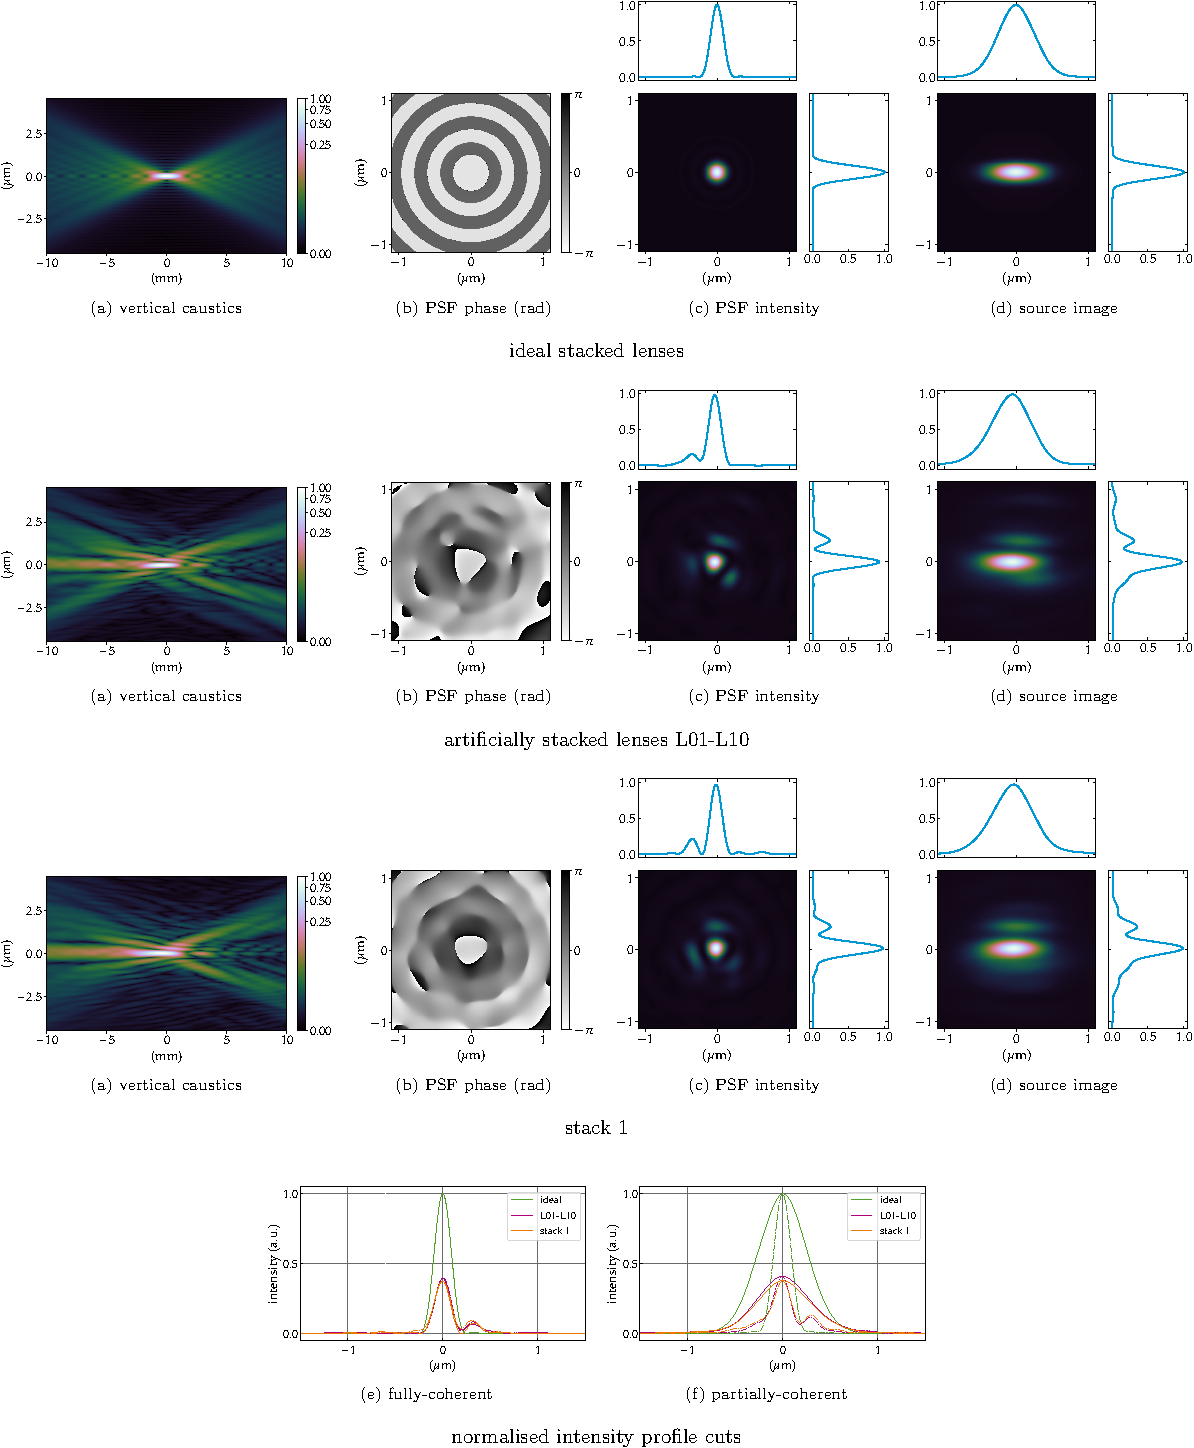
\includegraphics[width=1\linewidth]{figures/ch05/CDn_vs_CDnStack.pdf}}
        {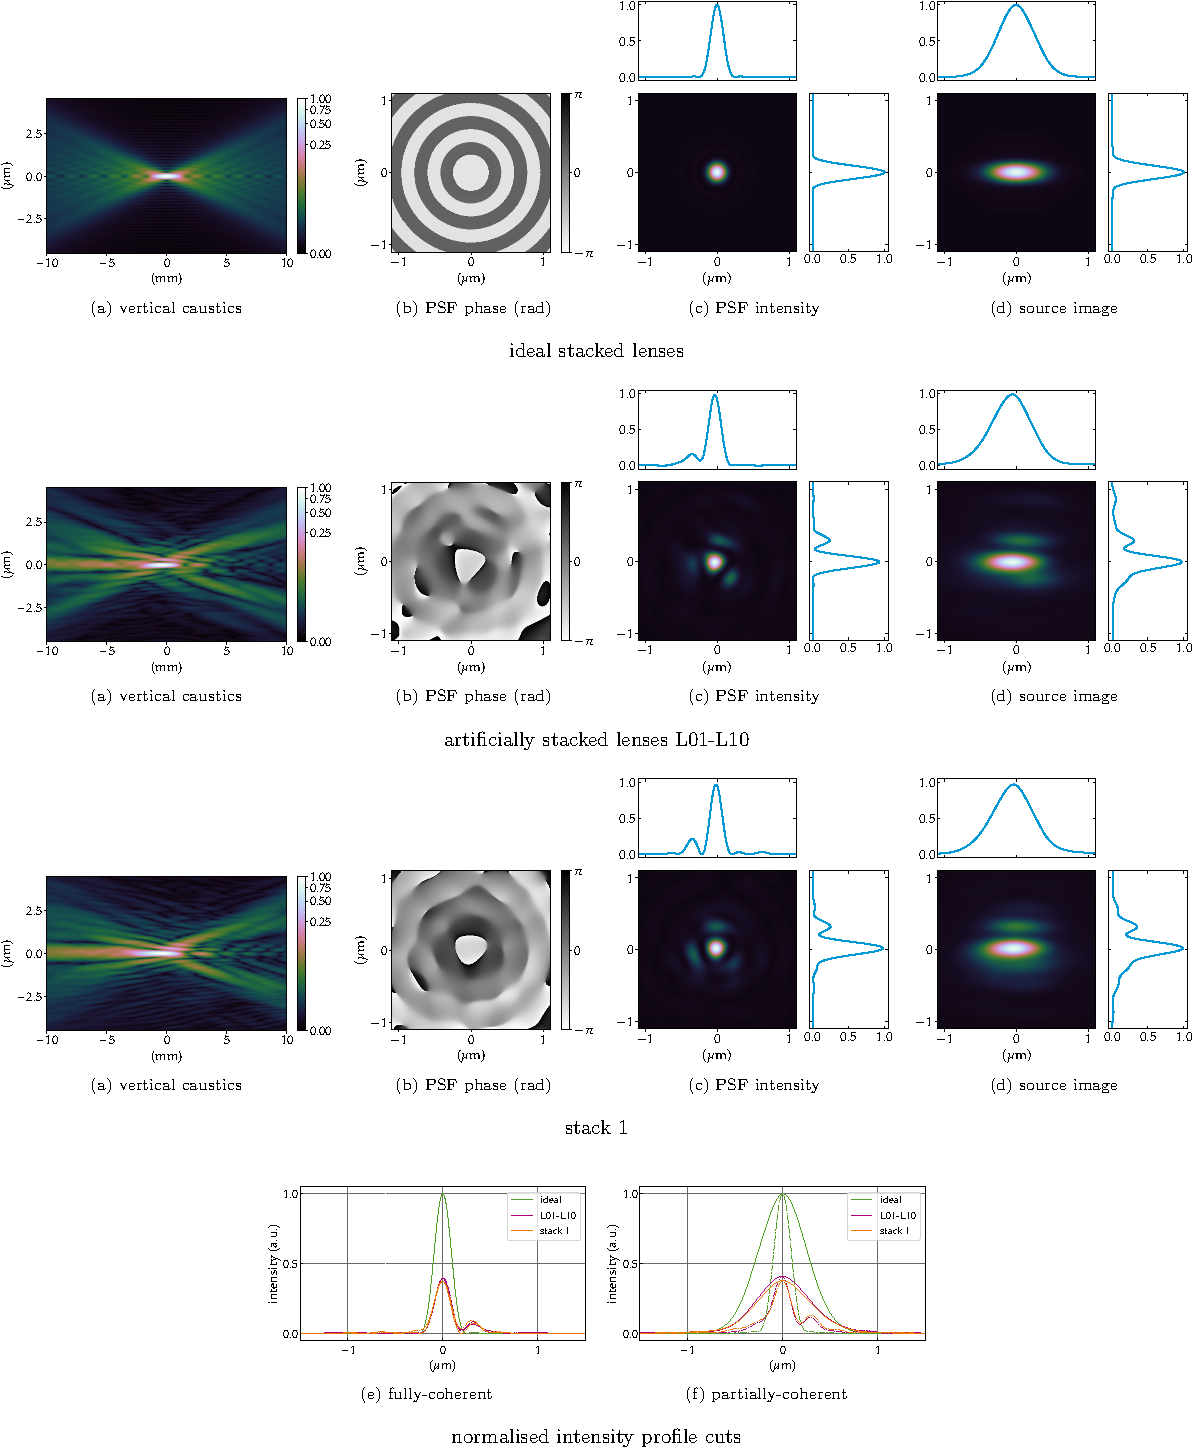
\includegraphics[width=1\linewidth]{figures/compressed/CDn_vs_CDnStack.pdf}}
        \caption[Artificially stacked lenses L01-L11 vs. stack 1 comparison]{Comparison between individually-measured lenses L01-L10 against the stack metrology of the same lenses. \textbf{top row}: ideal CRL, \textbf{upper middle row}: L01-L10 artificially stacked lenses measured individually. \textbf{lower middle row}: lenses measured as a stack. \textbf{bottom row}: horizontal (solid lines) and vertical (dashed lines) intensity cuts for coherent- and partially-coherent simulations. The simulated CRLs are composed of 10 2D-beryllium lens with nominal radius $R=50~\mu\text{m}$, geometric aperture $A_{\diameter}=440~\mu\text{m}$ and $t_\text{wall}=20~\mu$m at 8~keV. The error profiles used are the measured ones shown in Fig.~\ref{fig:accumulated_profile_1} and \ref{fig:CDn}.}\label{fig:CDn_vs_CDnStack}
\end{figure}

\begin{figure}[ht]
        \centering
        % {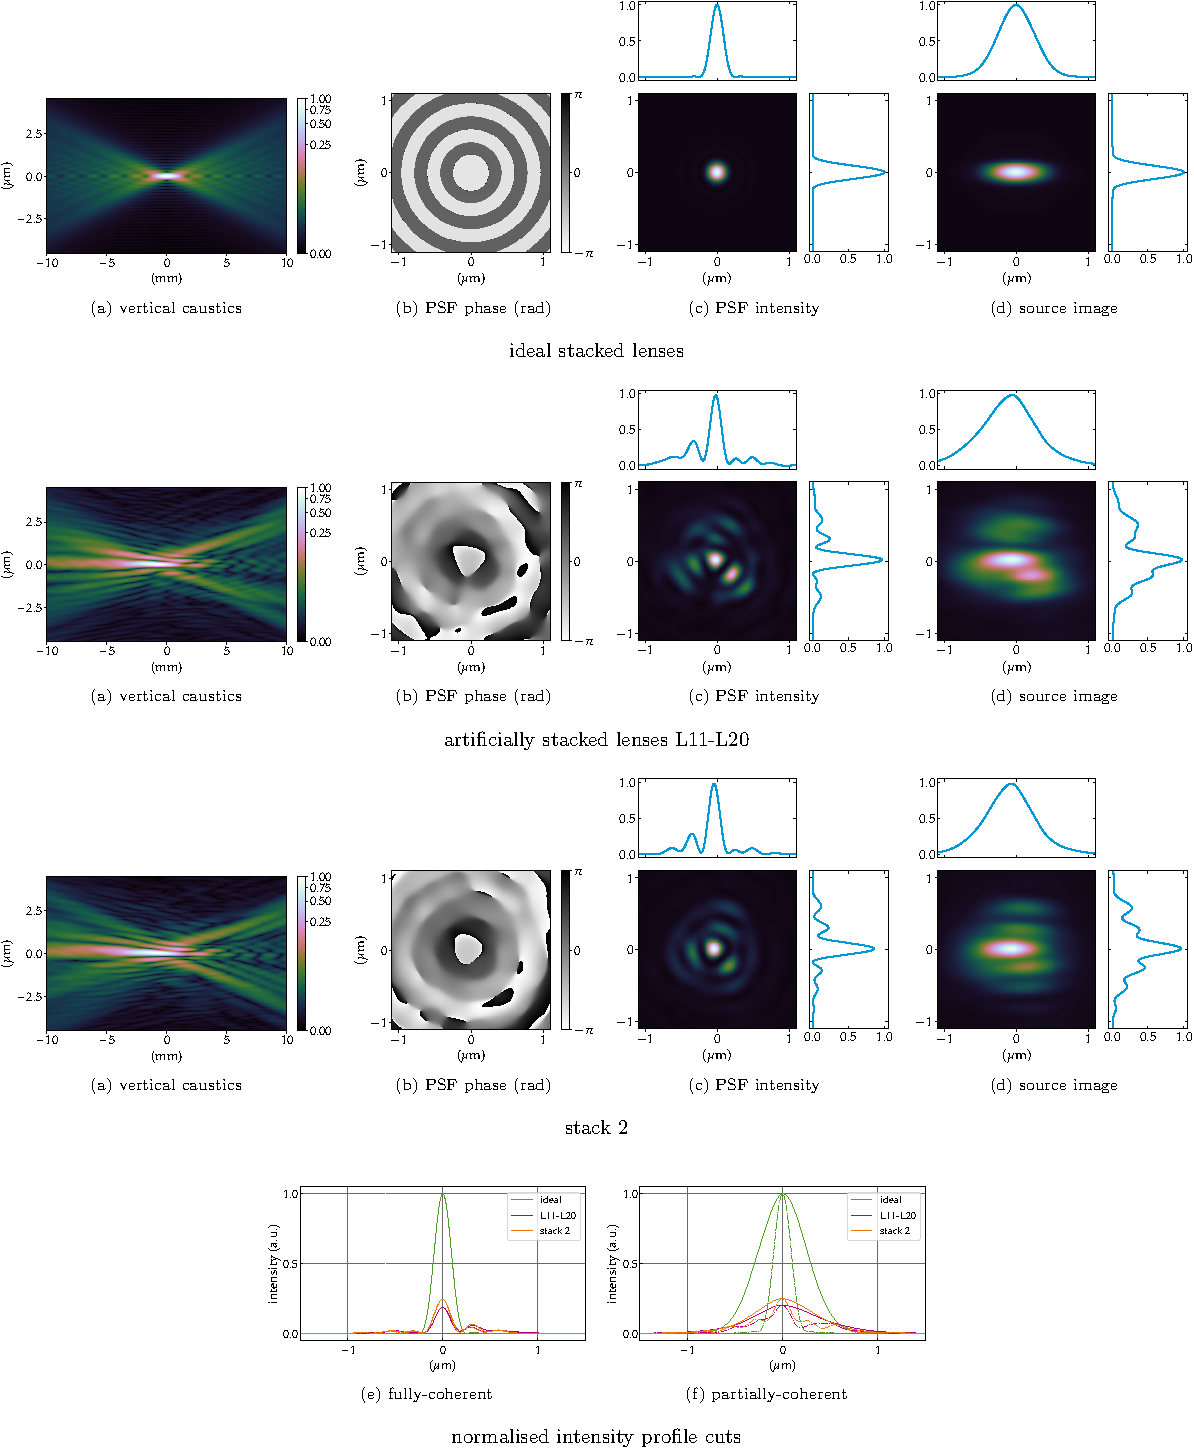
\includegraphics[width=1\linewidth]{figures/ch05/CDo_vs_CDoStack.pdf}}
        {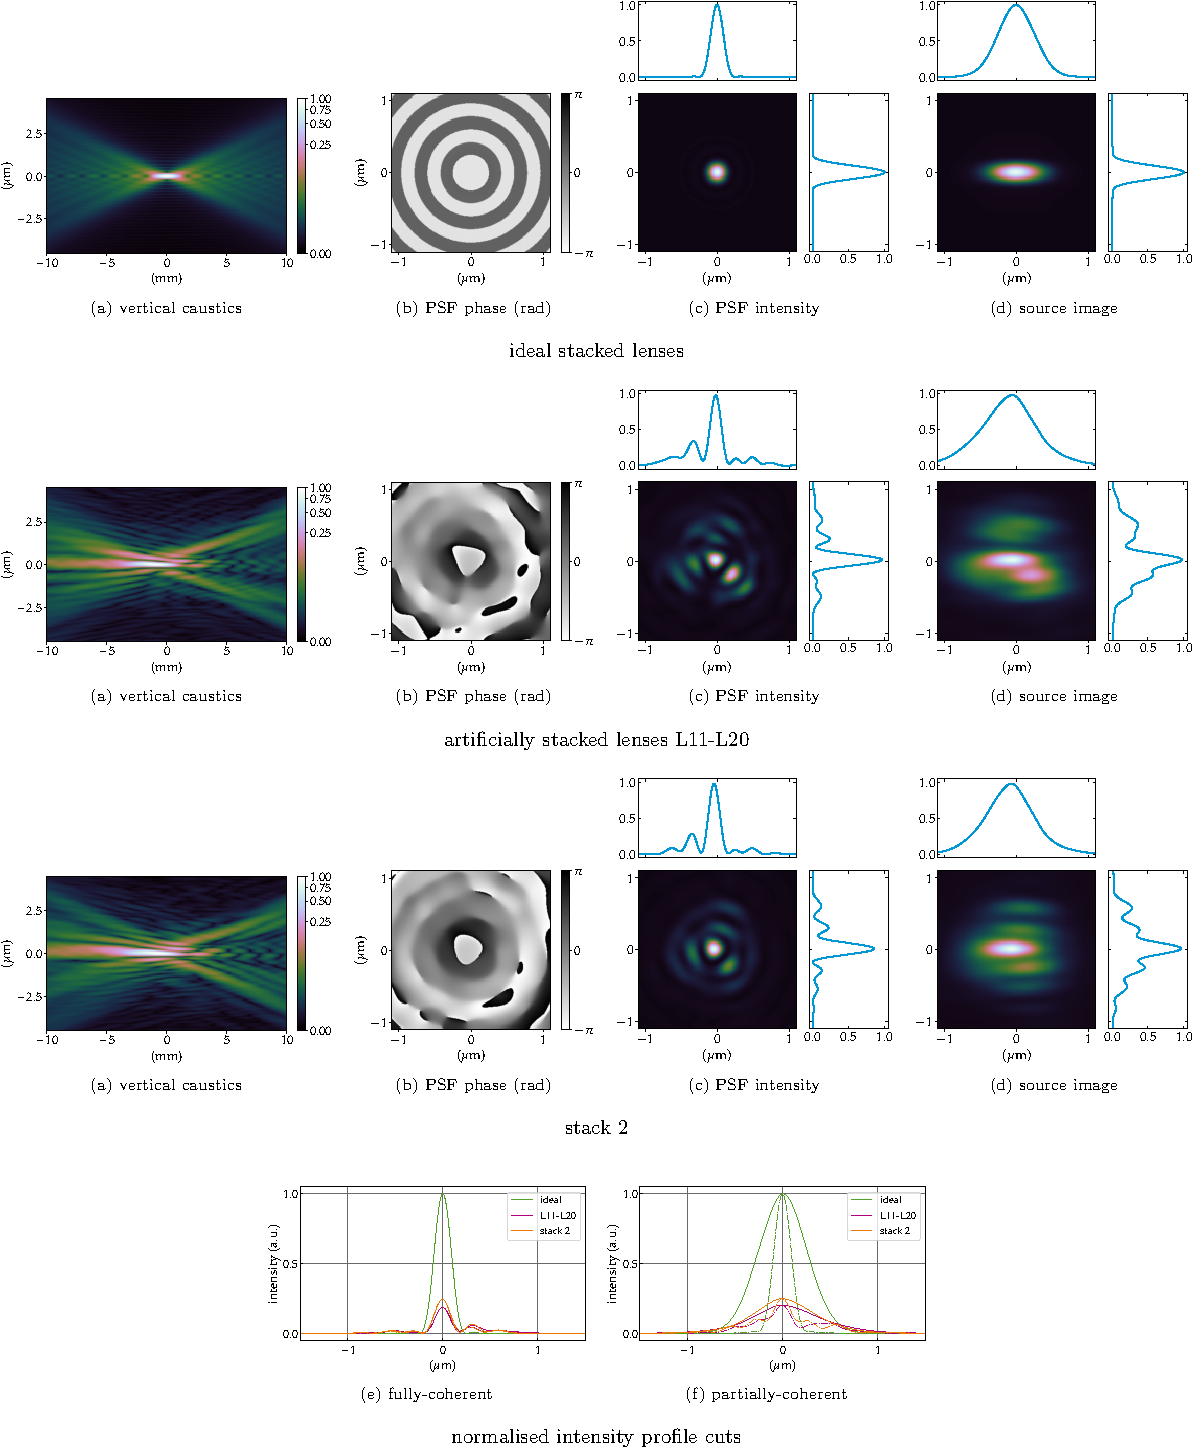
\includegraphics[width=1\linewidth]{figures/compressed/CDo_vs_CDoStack.pdf}}
        \caption[Artificially stacked lenses L11-L21 vs. stack 2 comparison]{Comparison between individually-measured lenses L11-L20 against the stack metrology of the same lenses. \textbf{top row}: ideal CRL, \textbf{upper middle row}: L11-L20 artificially stacked lenses measured individually. \textbf{lower middle row}: lenses measured as a stack. \textbf{bottom row}: horizontal (solid lines) and vertical (dashed lines) intensity cuts for coherent- and partially-coherent simulations. The simulated CRLs are composed of 10 2D-beryllium lens with nominal radius $R=50~\mu\text{m}$, geometric aperture $A_{\diameter}=440~\mu\text{m}$ and $t_\text{wall}=20~\mu$m at 8~keV. The error profiles used are the measured ones shown in Fig.~\ref{fig:accumulated_profile_2} and \ref{fig:CDo}.}\label{fig:CDo_vs_CDoStack}
\end{figure}

\begin{figure}[ht]
        \centering
        % {\includegraphics[width=1\linewidth]{figures/ch05/CDn01-05-10.pdf}}
        {\includegraphics[width=1\linewidth]{figures/compressed/CDn01-05-10.pdf}}
        \caption[Effects of stacking lenses]{Effects of artificially stacking individually measured lenses. \textbf{top row}: single L01 lens performance). \textbf{middle row}: L01-L05 artificially stacked lenses. \textbf{bottom row} L01-L10 artificially stacked lenses. The simulated CRLs are composed of 2D-beryllium lens with nominal radius $R=50~\mu\text{m}$, geometric aperture $A_{\diameter}=440~\mu\text{m}$ and $t_\text{wall}=20~\mu$m at 8~keV.}\label{fig:CDn01-05-10}
\end{figure}

\begin{figure}[ht]
        \centering
        % {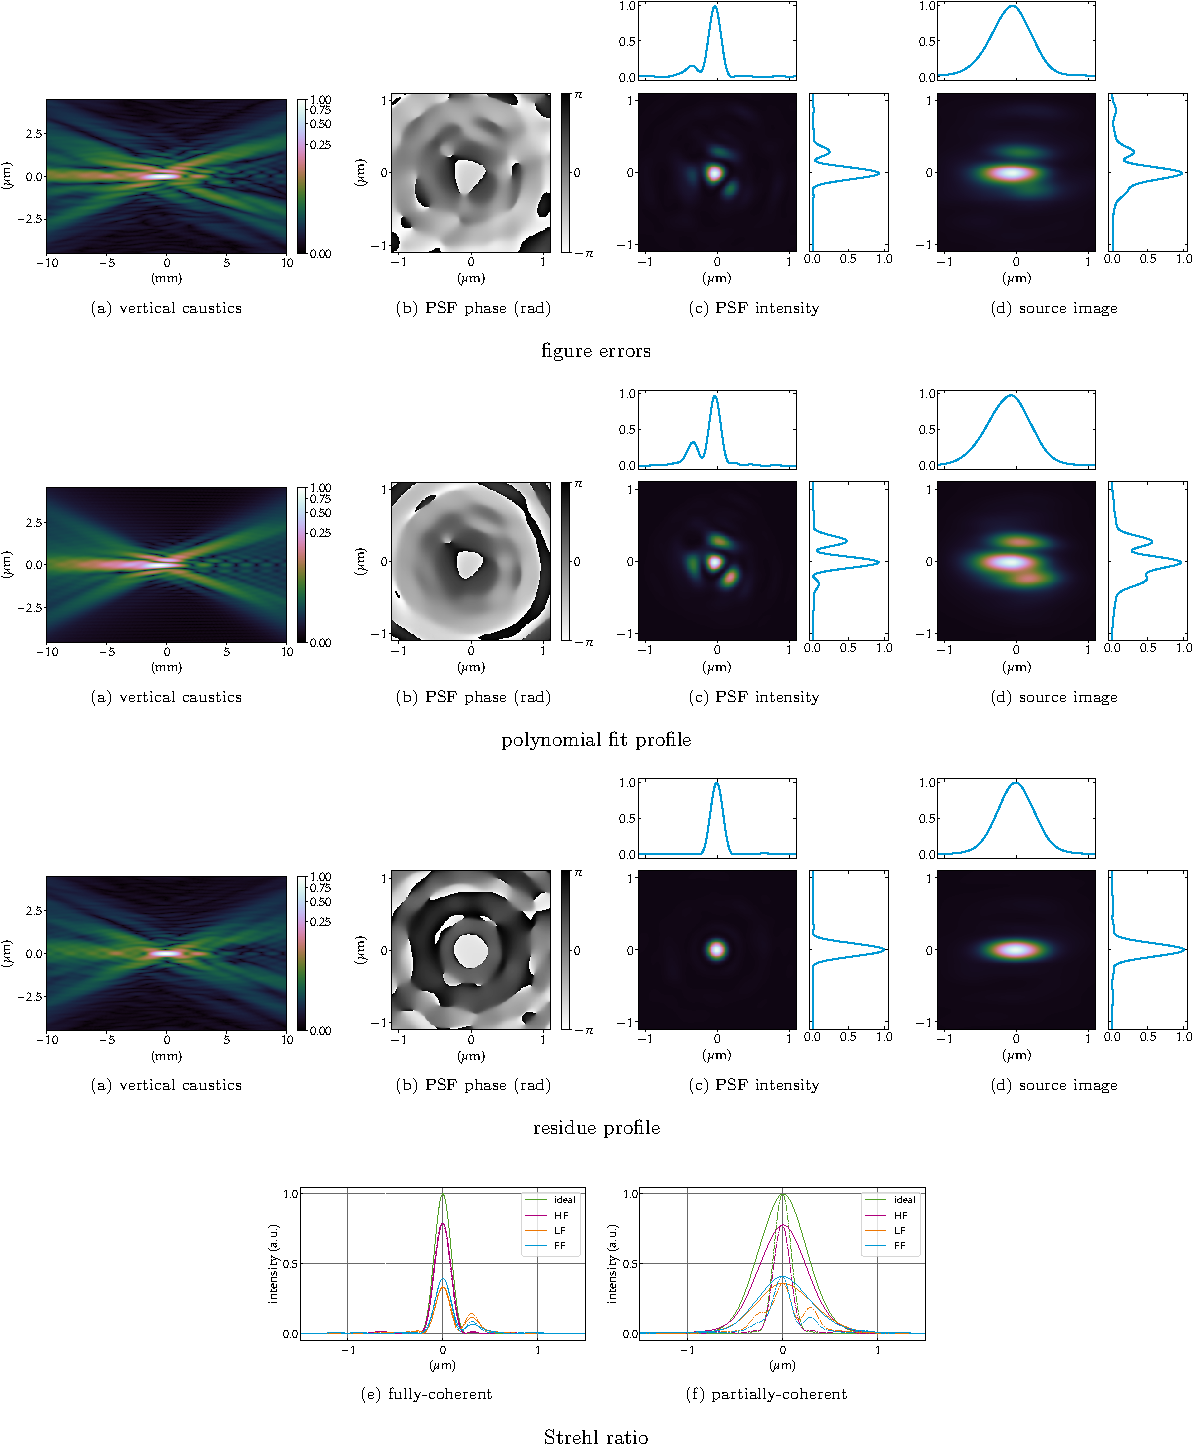
\includegraphics[width=1\linewidth]{figures/ch05/CDnFF_LF_HH.pdf}}
        {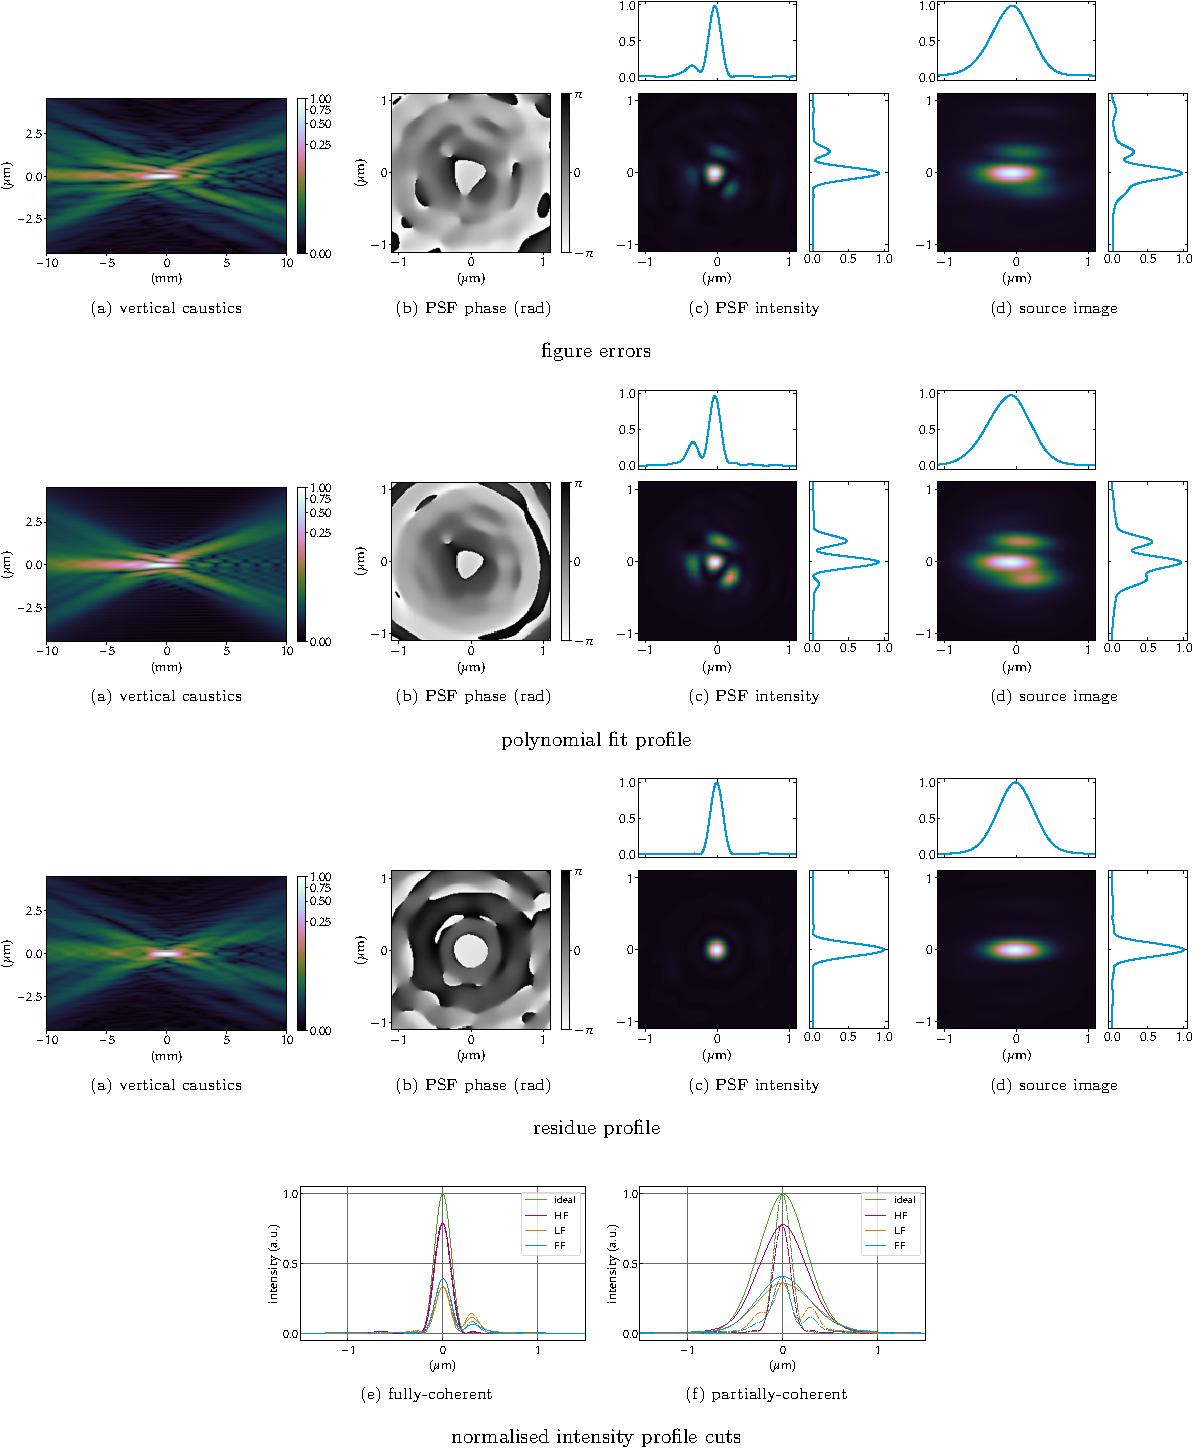
\includegraphics[width=1\linewidth]{figures/compressed/CDnFF_LF_HH.pdf}}
        \caption[Effects of different spatial frequencies ranges on a X-ray beam]{Effects of different spatial frequencies ranges on a X-ray beam. \textbf{top row}: full accumulated profile of individually measured and artificially measured L01-L10 lenses. \textbf{second row}: Zernike circle polynomial reconstruction of the accumulated profile. \textbf{third row}: residual profile from the fit added to ideal lenses. \textbf{bottom row}:($-$)  horizontal (solid lines) and vertical (dashed lines) intensity cuts for coherent- and partially-coherent simulations. The simulated CRLs are composed of 10 2D-beryllium lens with nominal radius $R=50~\mu\text{m}$, geometric aperture $A_{\diameter}=440~\mu\text{m}$ and $t_\text{wall}=20~\mu$m at 8~keV. The error profiles used are shown in Fig.~\ref{fig:accumulated_profile_1}.}\label{fig:CDnFF_LF_HH}
\end{figure}

\begin{figure}[ht]
        \centering
        % {\includegraphics[width=0.99\linewidth]{figures/ch05/CDn.pdf}}
        {\includegraphics[width=0.99\linewidth]{figures/compressed/CDn.pdf}}
        \caption[L01-L10 studied under fully- and partially-coherent illuminations]{Lens stack formed by individually measured lenses L01-L10 studied under fully- and partially-coherent illumination. (a) partially-coherent simulations show the beam profile up- and downstream the focal position averaging 10$^{4}$ wavefronts to simulate the radiation emitted by an undulator; (b) the coherent simulations show the beam profile of a plane wavefront being focused; (c) beam propagation near the focal position (beam caustics) for a fully coherent beam (horizontal cut around $y=0$); (d) phase and (e) intensity of the PSF calculated focusing a plane-wavefront; (f) demagnified image of the undulator photon-source (extended source). The simulated CRLs are composed of 10 2D-beryllium lens with nominal radius $R=50~\mu\text{m}$, geometric aperture $A_{\diameter}=440~\mu\text{m}$ and $t_\text{wall}=20~\mu$m at 8~keV. The error profiles used are shown in Fig.~\ref{fig:accumulated_profile_1}.}\label{fig:CDnS}
\end{figure}

\clearpage

% %-------------------------------------------------------------------------
% %-------------------------------------------------------------------------
% \section{Imaging}\label{sec:imaging_sim}
% %-------------------------------------------------------------------------
% %-------------------------------------------------------------------------
% \todo{If there's time: grid \& Siemens star [\cite{Simons2017}]} 

%-------------------------------------------------------------------------
%-------------------------------------------------------------------------
\section{Discussion}\label{sec:discussion}
%-------------------------------------------------------------------------
%-------------------------------------------------------------------------

The main results drawn from the simulations presented previously are discussed in this section. Firstly, some considerations on the effect of optical imperfections on a (partially) coherent X-ray beam are drawn. The merit of using the Strehl ratio for X-ray lens tolerancing is also discussed. Finally, some comments on the simulation times are presented.

%-------------------------------------------------------------------------
%-------------------------------------------------------------------------
\subsection{Metrology of individual lenses vs. stacked lenses}\label{sec:stacking}
%-------------------------------------------------------------------------
%-------------------------------------------------------------------------

The metrology of single lenses and that of lens stacks was already discussed in \S\ref{sec:metrology}~-~\textit{\nameref{sec:metrology}}. The qualitative agreement between the obtained profiles from the measurement of a lens stack and the individually measured and artificially stacked lenses is shown in Figs.~\ref{fig:accumulated_profile_1}-\ref{fig:CDo} and Tables~\ref{tab:CDn} and \ref{tab:CDo}. This qualitative agreement is confirmed by the simulations as shown in Figs.~\ref{fig:CDn_vs_CDnStack} and \ref{fig:CDo_vs_CDoStack}. Both sets of simulations, that is L01-L10 vs. stack 1 and L11-L20 vs. stack 2, show good agreement for the beam caustic, PSF and source image. The lenses L11-L20 and stack 2 show a lower degree of similarity in the partially-coherent simulation as shown in Fig.~\ref{fig:CDo_vs_CDoStack}(d). This can be attributed to the differences in the relative alignment of the lenses in the stack versus the lens holder in the individual measurements when performing the lenses metrology and subsequent software stacking. Figure~\ref{fig:CD_Strehl} shows the Strehl ratio for both coherent and partially-coherent simulations for both stacks. The coherent Strehl ratio shows very good agreement in terms of beam profile for both sets, despite the difference in intensity for the L11-L20 simulations. The L01-L10 simulations preserve the agreement on the partially-coherent simulations, but the L11-L20 set shows more difference between the individually measured lenses and the stack - see also Fig.~\ref{fig:CDo_vs_CDoStack}(d), but the general beam profile is maintained. When comparing the results in Fig.~\ref{fig:CD_Strehl} with the predicted Strehl ratios in Table~\ref{tab:Strehl}, a large discrepancy between the simulations of the L01-L10 lenses (individually measured and stack) is observed. It is predicted that the simulations using the metrology data from the lens stack (as opposed to the individually measured lenses) would have a much lower intensity due to a higher figure error value across the pupil, which is not observed. Although a deeper discussion on the Strehl ratio is presented in \S\ref{section:discussion_strehl}~-~\textit{\nameref{section:discussion_strehl}}, it is worth noting that the probable cause for this comes from the fact that the Strehl ratio predictions from Eqs.~\ref{eq:Strehl}-\ref{eq:Mahajan} were applied without weighing the errors with the beam transmission for this system - see Fig.~\ref{fig:EffectiveAperure}. The stack measurement has a smaller effective aperture due to the absorption and phase-contrast effects. The values of the figure errors towards the edge of the effective aperture are large and tend to be misrepresented when providing a single metric such as an RMS value for the figure error $\sigma_z$ over the full aperture. This, however, does not seem to be the case for the lens stack 2.

\begin{figure}[t]
    \centering
    {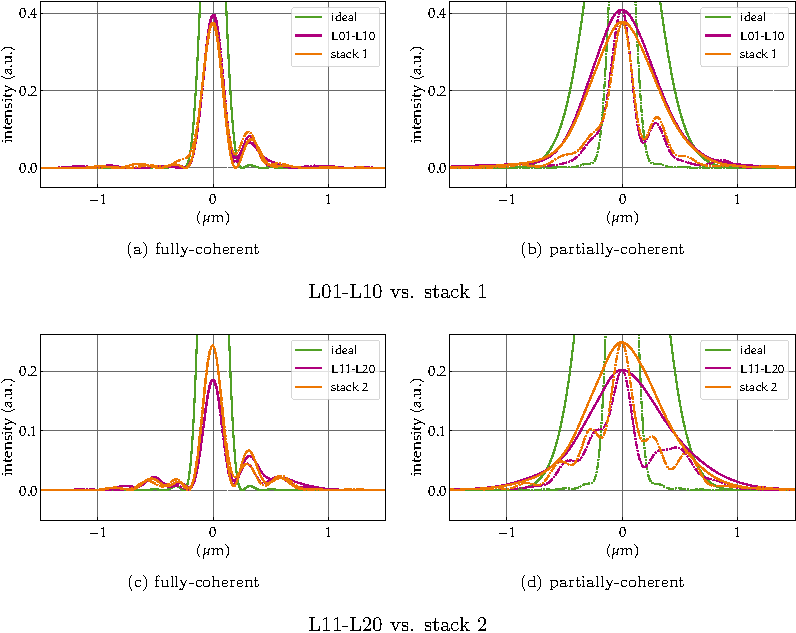
\includegraphics[width=0.75\linewidth]{figures/ch05/CD_Strehl.pdf}}
    \caption[Strehl ratio of L01-L10 vs. stack 1 and L11-L20 vs. stack 2 simulations]{Horizontal (solid lines) and vertical (dashed lines) intensity cuts for coherent- and partially-coherent simulations for the profiles in Figs.~\ref{fig:accumulated_profile_1}-\ref{fig:CDn} (\textbf{top row}) and the for the profiles in Figs.~\ref{fig:accumulated_profile_2} and \ref{fig:CDo} (\textbf{bottom row}) at 8~keV. }
    \label{fig:CD_Strehl}
\end{figure}

The effect on the resulting aberrations of stacking X-ray lenses has been modelled and discussed in depth by [\cite{Osterhoff2017}]. The progressive increase in the resulting figure errors from artificially stacked lenses is shown in Fig.~\ref{fig:stacking_errors}, which shows the evolution of the (a) full figure errors, (b) the polynomial fit of the full profile and (c) the residuals when stacking lenses. The simulations in Fig.~\ref{fig:CDn01-05-10} show the progressive deterioration of an X-ray beam by adding the figure errors to the simulations by showing three scenarios: a single lens, five lenses and ten lenses, representing a low-, a moderate- and a high-aberrated system. This sensitivity study is only possible because the metrology of individual lenses is available. Using the metrology of a full-stack and scaling it would not adequately represent the system due to the existence of correlated- and uncorrelated figure errors as pointed out by [\cite{Osterhoff2017}] and shown in Fig.~\ref{fig:stacking_errors}.

%  \todo{carefully read Osterhof's paper and make a comparison with his theory}.

\begin{figure}[t]
    \centering
    {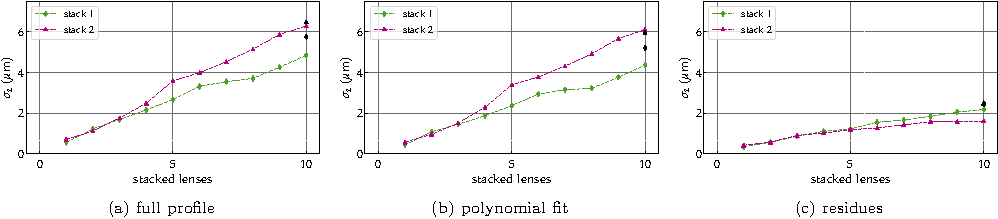
\includegraphics[width=1.\linewidth]{figures/ch04b/stacking_errors.pdf}}
    \caption[Accumulative figure errors]{Progressive increase of figure errors for the (a) full-, (b) fit- and (c) residual- profiles. The green-diamond shaped marker indicates the artificially stacked lenses from the stack 1, while the magenta triangles, the stack 2. The black markers indicate the corresponding measured stack. Figure errors calculated for a geometric aperture of $A_{\diameter}=400~\mu\text{m}$.}
    \label{fig:stacking_errors}
\end{figure}

%-------------------------------------------------------------------------
%-------------------------------------------------------------------------
\subsection{The effect of optical imperfections}\label{section:discussion_imperfections}
%-------------------------------------------------------------------------
%-------------------------------------------------------------------------

Applying the Mar\'echal criterion (Eq.~\ref{eq:MarechalCriterion}) calculated for beryllium lenses illuminated at 8~keV requires the accumulated projected figure errors to be $\sigma_z\leq2.08~\mu\text{m}$. Tables~\ref{tab:CDn} and \ref{tab:CDo} show that the accumulated thickness for both stacks is larger and that the optical system is operating far from ideal as the system exceeds the limit imposed by the Mar\'echal criterion. The decomposition of the figure error profiles into orthonormal polynomials and their resulting residuals is convenient because it allows investigating the effects of specific frequency ranges in the X-ray beam degradation. Following [\cite{Harvey1995a}], the figure errors of the lenses can be specified in terms of their spatial frequency, as they often have different effects on the image quality. Three regions are commonly used for that: low-, mid- and high-spatial-frequencies. The low-spatial frequencies (LF) are responsible for changing the beam profile and reducing the peak intensity. They are related to the conventional optical aberrations [\cite[\textit{\S9.1-3}]{born_wolf1999}] and they can be described by a set of orthonormal polynomials, which has been described in \S\ref{sec:orthonormal_polynomials}~-~\textit{\nameref{sec:orthonormal_polynomials}}. Mid- and high-spatial frequencies (HF) are responsible for scattering the light around the (focused) beam and have potential for broadening it, together with the expected reduction of the Strehl ratio. In this work, the mid- and high- frequencies are the residuals from the polynomial fit of the aberrated profile. The full profile comprises all spatial frequencies and is referred to as FF. From the analysis of the experimental data from 2D-beryllium lenses with nominal radius $R=50~\mu\text{m}$ and geometric aperture $A_{\diameter}=440~\mu\text{m}$, Zernike circle polynomials until the 37$^\text{th}$ order (3$^\text{rd}$ order spherical aberration) were used. Which causes the low-frequencies (LF) to span from $\sim500~\mu$m or $2\times10^{3}~\text{m}^{-1}$ (geometrical aperture of a lenslet) to $\sim50~\mu$m or $2\times10^{4}~\text{m}^{-1}$, while the mid- and high-frequencies span from $\sim50~\mu$m or $2\times10^{4}~\text{m}^{-1}$ to $\sim0.5~\mu$m or $2\times10^{6}~\text{m}^{-1}$, which is obtained from the Nyquist frequency of the measured data. Figure~\ref{fig:CDnFF_LF_HH} shows the effects of different spatial frequencies ranges on an X-ray beam. 

The addition of the mid- and high-spatial frequency errors to an ideal CRL model is related to scattering around the focused beam, contributing thus to increasing background and consequently reducing the peak intensity following [\cite{Harvey1995a}]. Using a linear scale, both the ideal PSF and the demagnified source image in Figs.~\ref{fig:CDn_vs_CDnStack}(c)-(d) are almost indistinguishable from their aberrated counterparts in Figs.~\ref{fig:CDnFF_LF_HH}(c)-(d), which is because the accumulated figure error complies to the Mar\'echal criterion. As pointed out by [\cite{Cocco2015, Cocco2019}], a high Strehl ratio does not guarantee a homogeneous beam profile up- and downstream of the focal position. This is apparent in the beam caustic shown in Fig.~\ref{fig:CDnFF_LF_HH}. The profile shown in Fig.~\ref{fig:CDn}(c) is not random and presents some concentric rings. This comes from the tooling of the punches used in the hot-embossing process of the Be lens fabrication. A more diverse profile, such as the one shown in Fig.~\ref{fig:CDnHF}, which also comes from the metrology of real Be lenses artificially stacked, allows to simulate the effects of a random HF error profile in the beam shape and its contribution to the scattering of light outside the beam envelope defined by the ideal beam caustics - this is shown in Fig.~\ref{fig:simulations_HF}. Comparing these simulations with the ones in Fig.~\ref{fig:CDnS} permits to say that the high-frequency errors lead to scattering of the beam and speckles, but generally, do not change the beam shape even away from the focal position.

When considering the low-spatial-frequency figure errors, however, the beam shape starts to change more drastically even at the focal position. The appearance of satellite peaks becomes pronounced in the PSF and the demagnified source image. The beam caustics start presenting an elongated tail-like structure upstream of the focal position and a ring-like structure downstream. The elongation of the beam along the optical axis and the presence of homogeneous concentric rings on the PSF are a classical signature of spherical aberration, which is a major component of the LF figure errors - cf. $Z_{11}$ in Figs.~\ref{fig:CDn}(d)-\ref{fig:accumulated_profile_2}(d). The predominance of spherical aberration on 2D parabolic Be lenses has already been observed; see Fig.~6.14 of [\cite{Seiboth2016b}]. The PSF due to spherical aberration can be seen also in Figs.~8.5 and 8.6 from [\cite{Mahajan2011}]. In the partially-coherent simulations, the satellite peaks around the main lobe seen at the PSF simulations are stretched horizontally to the point that their visibility is maintained vertically, but horizontal cuts (Fig.~\ref{fig:CDnFF_LF_HH}(d)) show almost no trace of them, due to the reduction in transverse horizontal coherence (blurring effect). Small misalignments between the lenslets and some residual tilt from the LF errors contribute to a lateral displacement of the beam in the image plane. Using the full-frequency-range figure errors yields a combined effect that is analogous to the superposition of the HF and LF figure errors. The complete set of simulations of the lenses L01-L10 using the CRL-MS modelling given by Eq.~\ref{eq:TE_CRL_MS_ERR} can be seen in Fig.~\ref{fig:CDnS}. The diffraction effects from the aperture of the CRL are not easily observable because the system has an apodised Gaussian intensity at the exit pupil [\cite{Mahajan1986}], but they contribute to the concentric ring structures seen on the ideal lenses simulation in Fig.~\ref{fig:CDnS}. In terms of wavefront preservation, X-ray lenses are more susceptible to the low-frequency figure errors, as they are the ones that change the beam profile up- and downstream the focal position. Fortunately, the low frequencies are those that can be readily corrected by the fitting of corrective optics - which will be discussed in \S\ref{sec:corrections}~-~\textit{\nameref{sec:corrections}}. 

\begin{figure}[t]
        \centering
        {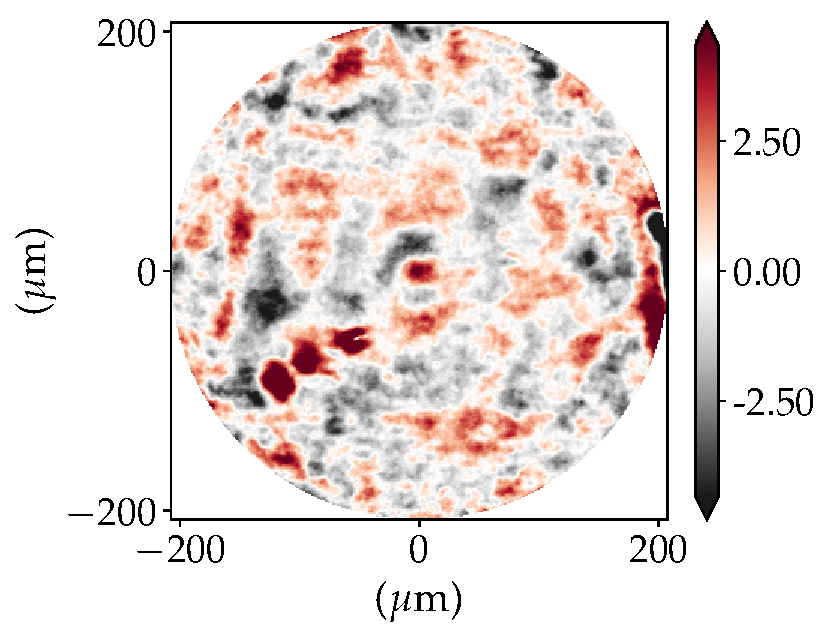
\includegraphics[width=0.3\linewidth]{figures/ch05/CDnHF/phase_n_CRL_errors_residues_phase_figure_errors_FF}}
        \caption[High frequency errors profile]{Artificially stacked high frequency error profile from 10 individually measure 2D-beryllium lens with nominal radius $R=50~\mu\text{m}$, geometric aperture $A_{\diameter}=440~\mu\text{m}$ and $t_\text{wall}=20~\mu$m used in the simulations shown in Fig.~\ref{eq:Strehl} and Fig.~\ref{fig:simulations_HF}. The profile has a $\sigma_z=1.74~\mu$m and the colour bar scale is in $\mu$m.}\label{fig:CDnHF}
\end{figure}

The simulations shown in Figs.~\ref{fig:CDn_vs_CDnStack} to \ref{fig:CDnS} paint a very consistent picture of the beam shape along the optical axis. Upstream of the image plane, a persistent central lobe is observed, albeit much less intense, with a high background around it thus reducing the signal to noise ratio. Downstream, the beam has a drop in intensity in the middle, looking like a doughnut when a cut transverse the optical axis is made. This behaviour is observed both on fully- and partially-coherent simulations and is more evident in the simulations shown in Fig.~\ref{fig:CDnS} (beam profiles). Such beam caustics have been extensively reported by experimental groups working under high coherent conditions, with similar optics and ptychographic reconstruction of X-ray beams - cf. Fig.~3 in [\cite{Schropp2013}], Fig.~2 in [\cite{Seiboth2016}], Fig.~3 in [\cite{Gasilov2017}] and Fig.~4 in [\cite{Seiboth2020}].



\clearpage 


\begin{figure}[t]
        \centering
        % {\includegraphics[width=0.99\linewidth]{figures/ch05/CDn_HF.pdf}}
        {\includegraphics[width=0.99\linewidth]{figures/compressed/CDn_HF.pdf}}
        \caption[High frequency errors studied under fully- and partially-coherent illuminations]{High frequency error profile studied under fully- and partially-coherent illumination. (a) partially-coherent simulations show the beam profile up- and downstream the focal position averaging 10$^{4}$ wavefronts to simulate the radiation emitted by an undulator; (b) the coherent simulations show the beam profile of a plane wavefront being focused; (c) beam propagation near the focal position (beam caustics) for a fully coherent beam (horizontal cut around $y=0$); (d) phase and (e) intensity of the PSF calculated focusing a plane-wavefront; (f) demagnified image of the undulator photon-source (extended source). The simulated CRLs are composed of 10 2D-beryllium lens with nominal radius $R=50~\mu\text{m}$, geometric aperture $A_{\diameter}=440~\mu\text{m}$ and $t_\text{wall}=20~\mu$m at 8~keV. The error profile used is shown in Fig.~\ref{fig:CDnHF}.}\label{fig:simulations_HF}
\end{figure}


\begin{figure}[t]
    \centering
    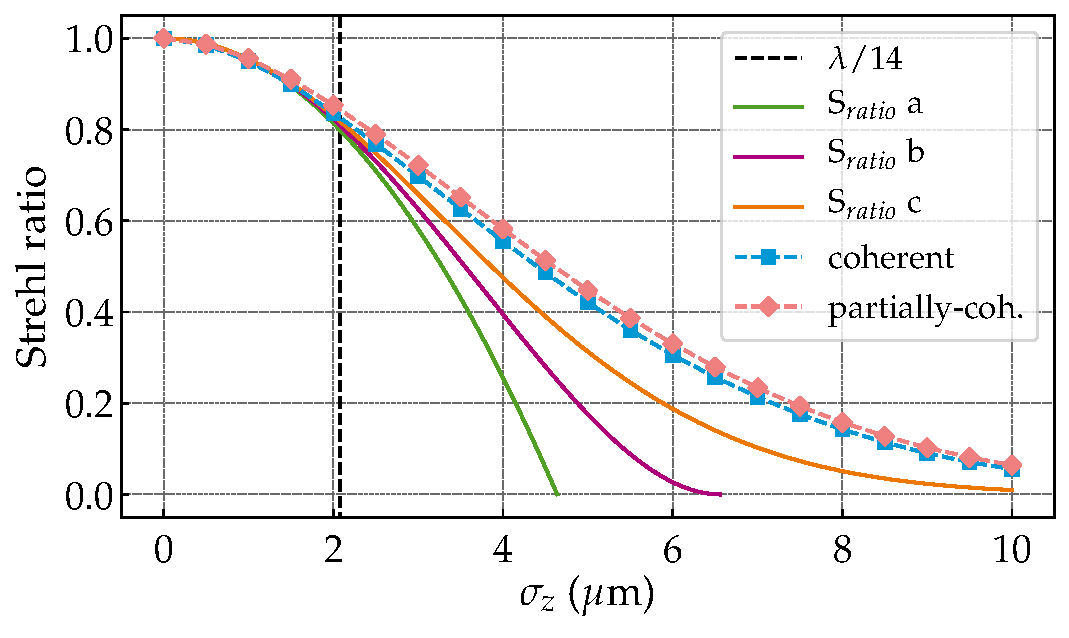
\includegraphics[width=7.5cm]{figures/ch05/fig_10.pdf} %trim = left bottom right top
    \caption[Strehl ratio from numerical simulations]{Strehl ratio from numerical simulations and from the application of different approximations (Eqs.~\ref{eq:Strehl}-\ref{eq:Mahajan}) as a function of the figure error $\sigma_z$ from a lens stack made of beryllium illuminated at 8~keV. The vertical dashed black line indicates the maximum tolerable thickness error (Eq.~\ref{eq:ThickLim}) for complying with the Mar\'echal criterion (Eq.~\ref{eq:MarechalCriterion}), that is, $\sigma_{\lambda/14}\approx2.08~\mu\text{m}$.}
    \label{fig:Strehl}
\end{figure}{}


\begin{figure}[ht]
    \centering
    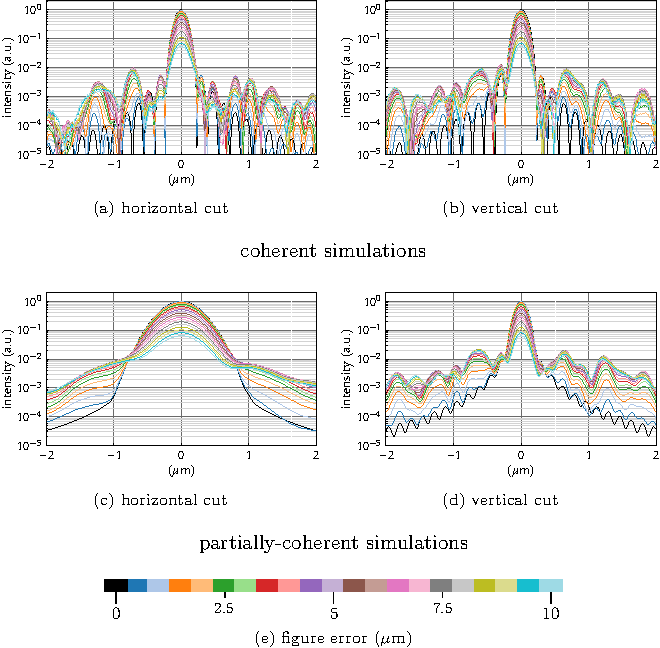
\includegraphics[width=0.7\linewidth]{figures/ch05/hf_strehl_scan.pdf} %trim = left bottom right top
    \caption[Intensity cut for $\sigma_z$ scan]{Intensity cuts as a function of the figure error $\sigma_z$ from a lens stack made of beryllium illuminated at 8~keV. The accumulated profile used presents predominantly the high-frequency content and is shown in Fig.~\ref{fig:CDnHF}. The associated Strehl ratio are shown in Fig.~\ref{fig:Strehl}. This spatial frequency range is related to scattering around the focused beam, contributing thus to increased background and consequently reducing the peak intensity.}
    \label{fig:hf_strehl_scan}
\end{figure}{}


%-------------------------------------------------------------------------
%-------------------------------------------------------------------------
\subsection{The Strehl ratio for X-ray lenses}\label{section:discussion_strehl}
%-------------------------------------------------------------------------
%-------------------------------------------------------------------------

The Strehl ratio for the CRL models is presented in Table~\ref{tab:Strehl}. In the numerical simulations, the intensity at the centre of the beam is normalised to the intensity obtained by the ideal model. What is generally observed is that for values lower than the  Mar\'echal criterion (Eq.~\ref{eq:MarechalCriterion}), the analytic equations Eqs.~\ref{eq:Strehl}-\ref{eq:Mahajan} show a good agreement and can be used to estimate the performance of an optical system close to the ideal performance. However, for moderate or strong values of aberrations the approximations used to derive those equations start to break down and other factors have to be taken into account, such as spatial distribution of the error profile and the transmission profile across the exit pupil. The values shown on Table~\ref{tab:Strehl} do not show a clear trend when it comes to the Strehl ratio and the RMS value of the figure error across the exit pupil of the system. In order to understand the numerically dependence of the Strehl ratio on the height error, each individual profile used to generate the profile shown in Fig.~\ref{fig:CDnHF} was scaled by a constant value to allow for a scanning of the total projected figure error $\sigma_z$. The results in Figure~\ref{fig:Strehl} show the expected Strehl ratio as a function of the projected figure errors $\sigma_z$ for different analytical approximations (Eqs.~\ref{eq:Strehl}-\ref{eq:Mahajan}) and for the numerical calculations with a fully- and partially-coherent illumination - these numerical calculations are also shown in Fig.~\ref{fig:hf_strehl_scan}. All approaches show very good agreement up to $S_\text{ratio}>0.8$, when they start diverging. The expressions for $S_\text{ratio a}$ (Eq.~\ref{eq:Strehl}) and  $S_\text{ratio b}$ (Eq.~\ref{eq:Marechal}) can be considered as approximations for $S_\text{ratio c}$ (Eq.~\ref{eq:Mahajan}), therefore are only expected to be valid over a restricted range (large $S_\text{ratio}$). A fit of the simulation data (coral rhombuses and blue squares in Fig.~\ref{fig:Strehl}) give:
\begin{subequations}\label{eq:Strhel_Exp_pre}
\begin{align}
    S_{\text{ratio coh.}}&\approx\exp{\big(-2.32\cdot10^{10}\sigma_z^2 -6.13\cdot10^4\sigma_z + 2.54\cdot10^{-2}\big)},\\
    S_{\text{ratio part.-coh.}}&\approx\exp{\big(-2.28\cdot10^{10}\sigma_z^2 -5.07\cdot10^4\sigma_z + 2.29\cdot10^{-2}\big)}.
\end{align}
\end{subequations}
Unfortunately, due to the nature of the projected figure errors (in the range of few micrometres r.m.s.), it is not possible to discard the non-quadratic terms. Equations~\ref{eq:Strhel_Exp_pre} can be rewritten as:
\begin{align}\label{eq:Strhel_Exp}
    S_{\text{ratio simulation}}&\approx\exp{\bigg[- \bigg(\frac{2\pi}{\lambda}\bigg)^2\big(\kappa_1\Delta\Phi\big)^2-\frac{2\pi}{\lambda}\kappa_2\Delta\Phi-\kappa_3\bigg]},
\end{align}
where $\kappa$ are scaling constants that, in principle, depend on the number of elements, lens material, energy and, mostly importantly, the spatial distribution of the accumulated errors over the optical element aperture. For our particular examples, $\kappa_1=0.71$, $\kappa_2=0.28$ and $\kappa_3=2.54\cdot10^{-2}$ for the coherent case and $\kappa_1=0.70$, $\kappa_2=0.24$ and $\kappa_3=2.29\cdot10^{-2}$ for the partially-coherent case. When comparing Eq.~\ref{eq:Strhel_Exp} with Eq.~\ref{eq:Mahajan}, a $\kappa<1$ suggests that there is some weighting of the phase errors reducing their effect, but simply multiplying the accumulated thickness errors (cf. Figs.~\ref{fig:CDn}-\ref{fig:accumulated_profile_2}) with the normalised optical system transmission (cf. Fig.~\ref{fig:EffectiveAperure}) does not allow prediction of $\kappa$ and this is still as an open question at the time of writing, which strengths the case for the simulation framework developed for this thesis.

% \begin{table}[b]
% \caption[Summary of the simulation times for different CRL models]{Summary of the simulation times for different CRL models. From the most simple one (single lens equivalent) up to the more complex multi-slicing (MS) with figure errors. Simulations were performed on a Intel(R) Xeon(R) CPU E5-2680 v4 @ 2.40GHz cluster at the ESRF. Partially coherent calculations were done using 28 cores in parallel.}\label{tab:simulation_time}\small
% \centering
% \begin{tabular}{rccc}\hline\hline
% \multicolumn{1}{c}{\textbf{model}} & \textbf{fully coherent} &\textbf{ partially coherent} & \textbf{caustics}\\\cline{1-4}
% single lens equivalent (Eq.~\ref{eq:TE_CRL})                 &33~s            &2~h~44~min  &1~h~32~min               \\
% multi-slicing  (Eq.~\ref{eq:TE_CRL_MS})                     &58~s            &5~h~12~min  &1~h~33~min               \\
% MS + figure errors  (Eq.~\ref{eq:TE_CRL_MS_ERR})                &2~min~48~s      &5~h~42~min  &1~h~35~min               \\\cline{2-4}
% \multicolumn{1}{c}{}               & (1 wavefront)  & (10$^{4}$ wavefronts)  & (4001 pts.) \\\hline\hline
% \end{tabular}
% \end{table}

%-------------------------------------------------------------------------
%-------------------------------------------------------------------------
\subsection{Simulation time}\label{section:discussion_time}
%-------------------------------------------------------------------------
%-------------------------------------------------------------------------

Increasing the complexity of the simulation model comes at the expense of increasing the overall simulation time, but as long as the transverse wavefront sampling is maintained, memory consumption is not affected from one model to another. The time increase in the simulations is mainly due to: \textit{i}) increase in the number of drift spaces and the number of optical elements; \textit{ii}) from reading the densely sampled metrology data. Table~\ref{tab:simulation_time} presents the typical simulation times for this work. Those are particularly high because the transverse sampling of the wavefronts is several times larger than the nominal minimal sampling necessary to mitigate artefacts or under-resolved features on the wavefront. Employing 10$^{4}$ wavefronts for the partially coherent simulations is also exaggerated but was done to ensure that any changes on the simulation come from the change of model being studied and not from statistical nature of the sampling of the electron-beam phase-space. The simulation times presented on Table~\ref{tab:simulation_time} can be certainly be reduced without loss of accuracy by adopting a more sensible sampling. $\blacksquare$

\begin{table}[h]
\caption[Summary of the simulation times for different CRL models]{Summary of the simulation times for different CRL models. From the most simple one (single lens equivalent) up to the more complex multi-slicing (MS) with figure errors. Simulations were performed on a Intel(R) Xeon(R) CPU E5-2680 v4 @ 2.40GHz cluster at the ESRF. Partially coherent calculations were done using 28 cores in parallel.}\label{tab:simulation_time}\small
\centering
\begin{tabular}{rccc}\hline\hline
\multicolumn{1}{c}{\textbf{model}} & \textbf{fully coherent} &\textbf{ partially coherent} & \textbf{caustics}\\\cline{1-4}
single lens equivalent (Eq.~\ref{eq:TE_CRL})                 &33~s            &2~h~44~min  &1~h~32~min               \\
multi-slicing  (Eq.~\ref{eq:TE_CRL_MS})                     &58~s            &5~h~12~min  &1~h~33~min               \\
MS + figure errors  (Eq.~\ref{eq:TE_CRL_MS_ERR})                &2~min~48~s      &5~h~42~min  &1~h~35~min               \\\cline{2-4}
\multicolumn{1}{c}{}               & (1 wavefront)  & (10$^{4}$ wavefronts)  & (4001 pts.) \\\hline\hline
\end{tabular}
\end{table}

% \clearpage

\addcontentsline{toc}{section}{References}
\printbibliography[heading=subbibliography]
\end{refsection}

